\section{Experiments}\label{sec:experiment}



We experimentally evaluated our approach. In the following of this section, we first present the testing infrastructure adopted in our experiments,
then we discuss the experimental settings, and
finally we discuss the performance of our heuristic algorithm.

\subsection{Testing Infrastructure and Experimental Settings}
Our testing infrastructure is a Python-based simulator of a complete service-based ecosystem, including service execution, comparison, and composition. The simulator is used to assess the performance and quality of our sliding window heuristic in Section \ref{sec:} for the generation of the best pipeline instance (Section \ref{sec:}). Performance measures the heuristics execution time in different settings, while quality compares the results provided by our heuristics in terms of selected services with the optimal solution retrieved using the exhaustive approach.
%We note that the exhaustive approach generates the best pipeline instance by executing all possible combinations of candidate services.
%The emulator simplifies the execution of the service composition by removing the service selection phase, which is not relevant for the purpose of the experiment.
Our experiments have been run on a workstation equipped with a 2.40GHz i5-8279U CPU with 16GB RAM and a 512GB SSD.

SETTING

\subsection{Perfomance}
% \subsection{performance}
% \begin{itemize}
%   \item Finestra scorrevole da 1 a N=Nodi
%   \item Servizi 5 a 20 passo 5 + 50??
%   \item
% \end{itemize}
% \subsection{Metriche/Euristiche}

The procedure was repeated by varying only one service at a time and executing the entire pipeline.
The experiments were primarily evaluated along three dimensions:

(i) Evaluation of the exhaustive execution time of all combinations by incrementing the number of services and nodes periodically:
This experiment aimed to comprehend how execution time fluctuates with increasing numbers of nodes and services.
The number of nodes was varied from 1 to 6, while the number of services was varied from 2 to 20, with a step of 1.
The execution has been stopped at the first combination that reported an execution time greater than 10k seconds.
The observed trend aligns with expectations, exhibiting exponential growth in execution times as the number of nodes increases.

Refer to Table X for a graphical representation.

(ii) Evaluation of execution time with the introduction of heuristics:
The heuristics, as defined in the relevant section, were incorporated,
and the entire pipeline was rerun with variations in the number of nodes,
services, and the size of the sliding window.

Notably, a window of size 1 corresponds to a greedy algorithm execution,
while a window of size n, where n is the number of nodes, is analogous to exhaustive execution.

(iii) Comparison of the optimal versus heuristics:
The optimal combination, characterized by the least data loss in the execution of the entire pipeline,
was determined by computing the minimum coefficient of variation for each combination.
The computation of the optimum necessitates exhaustive execution, involving all possible combinations of candidate services at each node.
Heuristics reduce execution time by approximating this selection through the use of a sliding window and generating all combinations within the window.
The objective of this final experiment is to assess the disparity between the optimum obtained with the sliding window and that obtained through exhaustive execution.

To introduce a level of interdependence among services,
matrices containing the degrees of dependence of each service with the next were employed.
It is important to note that different definitions of the optimum may yield slightly different results.

\begin{figure}
  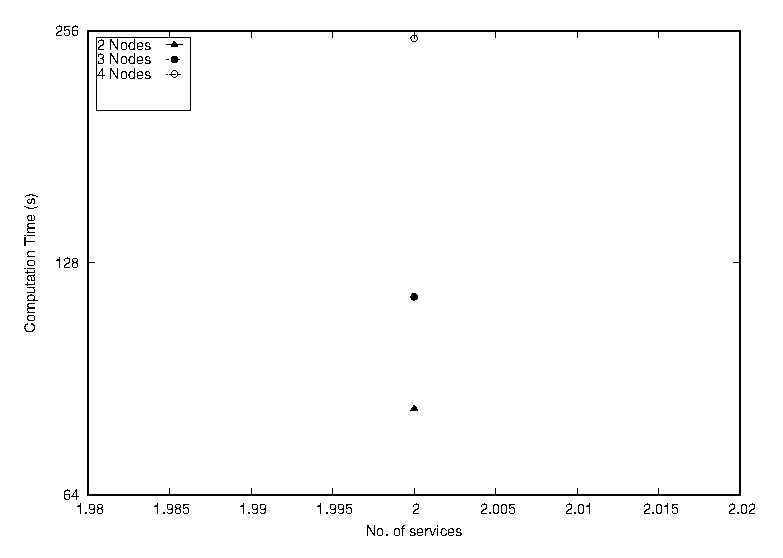
\includegraphics[width=0.95\columnwidth]{graphs/exhaustive_performance.eps}
  \caption{Preliminary performance evaluation.}
  \label{fig:perf_exhaustive}
\end{figure}
\begin{figure*}
  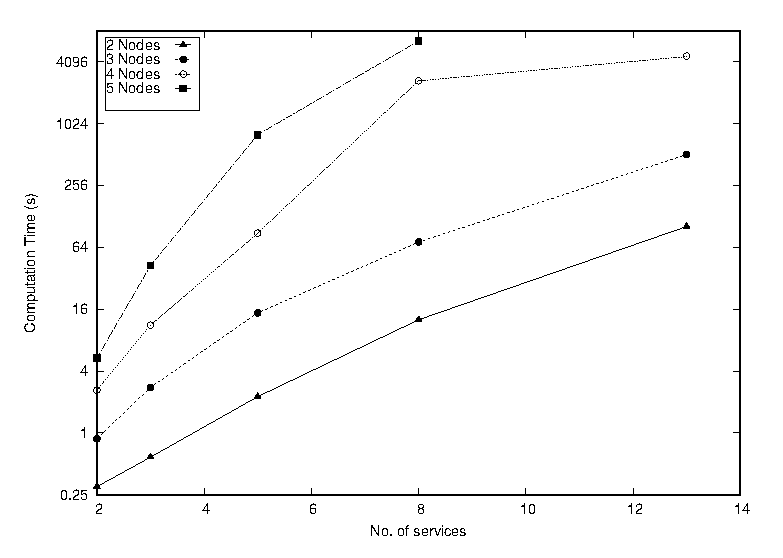
\includegraphics[width=0.95\textwidth]{graphs/window_performance.eps}
  \caption{Preliminary performance evaluation.}
  \label{fig:perf_window}
\end{figure*}


\usetikzlibrary{positioning}
\usetikzlibrary{backgrounds}



\begin{figure}[ht!]
  \centering
  \newcommand{\function}{$\instanceChartAnnotation{}$}
  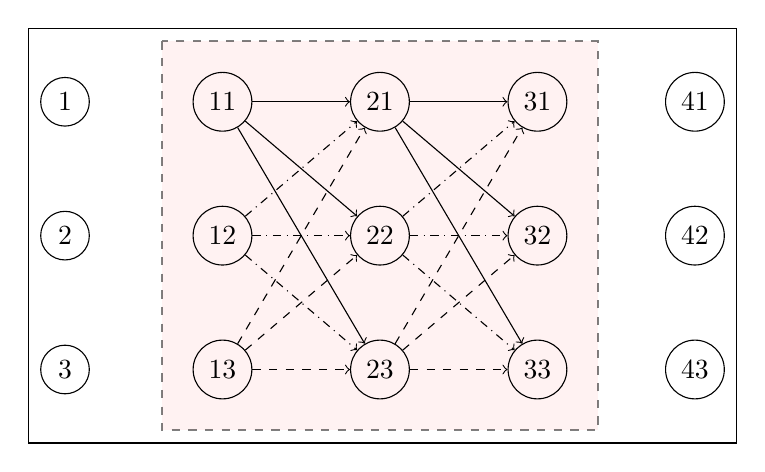
\begin{tikzpicture}[framed]
    \node[draw, circle] (s41) at (1,1.7) {$\sii{1}$};
    \node[draw, circle] (s42) at (1,0) {$\sii{2}$};
    \node[draw, circle] (s43) at (1,-1.7) {$\sii{3}$};

    \node[draw, circle] (s1) at (3,1.7) {$\sii{11}$};
    \node[draw, circle] (s2) at (3,0) {$\sii{12}$};
    \node[draw, circle] (s3) at (3,-1.7) {$\sii{13}$};

    \node[draw, circle] (s11) at (5,1.7) {$\sii{21}$};
    \node[draw, circle] (s12) at (5,0) {$\sii{22}$};
    \node[draw, circle] (s13) at (5,-1.7) {$\sii{23}$};

    \node[draw, circle] (s21) at (7,1.7) {$\sii{31}$};
    \node[draw, circle] (s22) at (7,0) {$\sii{32}$};
    \node[draw, circle] (s23) at (7,-1.7) {$\sii{33}$};

    \node[draw, circle] (s31) at (9,1.7) {$\sii{41}$};
    \node[draw, circle] (s32) at (9,0) {$\sii{42}$};
    \node[draw, circle] (s33) at (9,-1.7) {$\sii{43}$};


    % \draw[->] (node2) -- (node3);
    \draw[->] (s1) -- (s11);
    \draw[->] (s1) -- (s12);
    \draw[->] (s1) -- (s13);

    \draw[->,dashdotted] (s2) -- (s11);
    \draw[->,dashdotted] (s2) -- (s12);
    \draw[->,dashdotted] (s2) -- (s13);

    \draw[->,dashed] (s3) -- (s11);
    \draw[->,dashed] (s3) -- (s12);
    \draw[->,dashed] (s3) -- (s13);


    \draw[->] (s11) -- (s21);
    \draw[->] (s11) -- (s22);
    \draw[->] (s11) -- (s23);

    \draw[->,dashdotted] (s12) -- (s21);
    \draw[->,dashdotted] (s12) -- (s22);
    \draw[->,dashdotted] (s12) -- (s23);

    \draw[->,dashed] (s13) -- (s21);
    \draw[->,dashed] (s13) -- (s22);
    \draw[->,dashed] (s13) -- (s23);


    \begin{scope}[on background layer]
      \draw[thick, dashed, fill=red!10, opacity=0.5]
      ([shift={(-0.5,0.5)}]s1.north west) rectangle ([shift={(0.5,-0.5)}]s23.south east);

    \end{scope}
  \end{tikzpicture}
  \caption{Service composition instance}
  \label{fig:service_composition_instance}
\end{figure}
\subsection{Quality}
